\documentclass[12pt,oneside]{article}
\newcommand{\name}{Jean-Yves Djamen}
\newcommand{\class}{Math 80266A}
\newcommand{\hwnumber}{2}

\usepackage[margin=1in,letterpaper]{geometry}
%geometry changes the margins
%inside straight bracket is a parameter, inside curly bracket is name of package or whatever
%

\usepackage{amssymb,amsthm,amsmath,enumerate,fancyhdr,graphicx,tabularx}
\usepackage{float}
\usepackage{microtype}
\usepackage{tikz}
%Enables Graph Theory
\usepackage{pgfplots}
\usepackage{mdframed}
\usepackage[T1]{fontenc}
%Draws fancy boxes
\usepackage{parskip}
%Paragraph skip
\linespread{1.1} 
%Space in between lines
\usepackage{sectsty}
\sectionfont{\fontsize{12}{15}\selectfont}

\newenvironment{problem}[1]
{\begin{mdframed}
%Frames and crap
        \textbf{\textsc{Problem #1:}}
}
{\end{mdframed}}


\newenvironment{solution}
    {\textbf{\textsc{Solution:}}\\}
    {\newpage}

\pgfplotsset{compat=1.16}
\pagestyle{fancy}
\lhead{\textbf{\name}}
\chead{}
\rhead{\textbf{\class\ Assignment\ \hwnumber}}
\rfoot{\thepage}
\cfoot{}
\renewcommand{\headrulewidth}{0.2pt}

%lhead is the left header
%/textbf is text bold header

\def\l{\ell}
\def\pt{\partial}
\def\fish{\mathcal{I}}
\begin{document}

% \begin{enumerate}[I.]
% \item Solution number 1
% \item Solution Dos
% \item 
% \end{enumerate}

%/includgraphics

%/begin{align*}
%Stuff in here
%If star isn't included then the align command will automatically number your crap
%/end{align*}


\begin{problem}{}
Carry out a small simulation study to investigate the coverage of two-sided confidence intervals (CI) for return levels of a generalized extreme value (GEV) distribution based on
\begin{itemize}
    \item the delta method and asymptotic properties of MLE;
    \item the profile likelihood.
\end{itemize}
More specifically,
\begin{itemize}
    \item Generate samples of size n from a GEV. Consider $n = 50$ and $n = 100$.
    \item Check the coverage of the ($1 - \alpha$)100\% CI for $z_p$. Consider $\alpha$ = 0.05 and p = 0.001, 0.01.
\end{itemize}
Results based on 1000 simulations for each setting should be sufficient. The settings should
be chosen judiciously and you need to justify your choices. A reminder that two-sided CI
have the same probability of missing on the left as on the right. Your study and comments
should also address this issue.
\end{problem}

\begin{solution}
First, we observe that the nature of our task restricts the values of $\xi$ we can use in our settings. Below is a table outlining the experiments and the chosen parameters.
\begin{center}
    \begin{tabular}{||c|c|c|c|c|c|c|}\hline
     Experiment& $\xi$ & $\mu$&$\sigma$ &$n$ &$p$&$G(z_p)$ \\\hline
     I& 0.3 & 100 & 10 & 50 & 0.001&0.999\\\hline
     II&0.3  & 100 & 10 & 50 & 0.01&0.99 \\\hline
     III& 0.3 &0  &1  & 100 & 0.001&0.999\\\hline
     IV& 0.3 &  0&  1& 100 & 0.01&0.99\\\hline
\end{tabular}
\end{center}
Our choice of $\xi>0$ here means that our simulated data will behave similarly to data drawn from the Fréchet maximal domain of attraction. In fact, it means that there is no upper bound on the input to the pdf of the given GEV. This should mean that we should see some fairly large values for $z_p$ at $p=0.999$.  Furthermore, by picking $\xi>-0.5$ we have ensured that the MLE is regular and we can apply normality assumptions when retrieving the confidence interval for $z_p$ through the delta method. Different values of $\mu,\sigma$ were chosen mostly to experiment with the effects of location and scale changes. When working with $n=100$, we surmised that having a ``standardized" location and scale of 0,1 (respectively) would limit some of the errors arising from the numerical approaches used in the experiments.

\section*{Experiment I}
\begin{figure}[H]
\begin{center}
{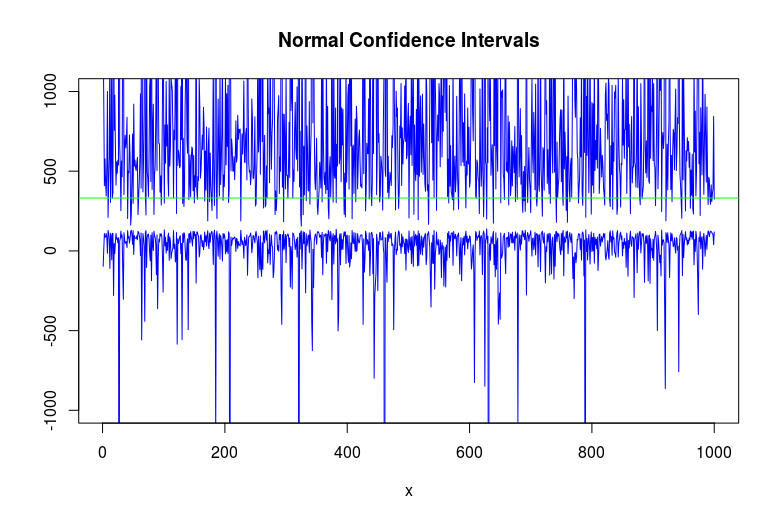
\includegraphics[width=3in]{Assignments/a2/e1-nci.png}}
{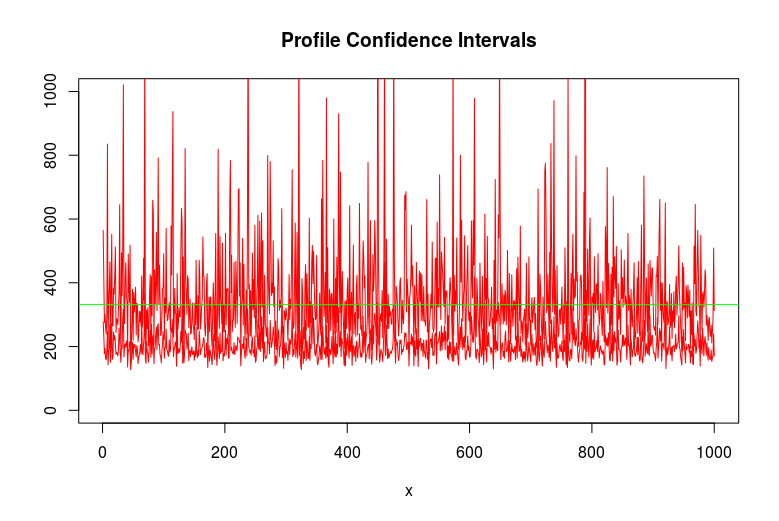
\includegraphics[width=3in]{Assignments/a2/e1-pllci.png}}
\caption{Experiment I confidence intervals for $z_p$(green) given through MLE (blue) and profile likelihood (red) methods. We see poorer coverage from the profile likelihood intervals. In the graphs above, we note that the upper bounds for any of the intervals tend to be quite large. This is because we are estimating the $0.999^{th}$ quantile.}
\end{center}
\end{figure}
 
\section*{Experiment II}
\begin{figure}[H]
\begin{center}
{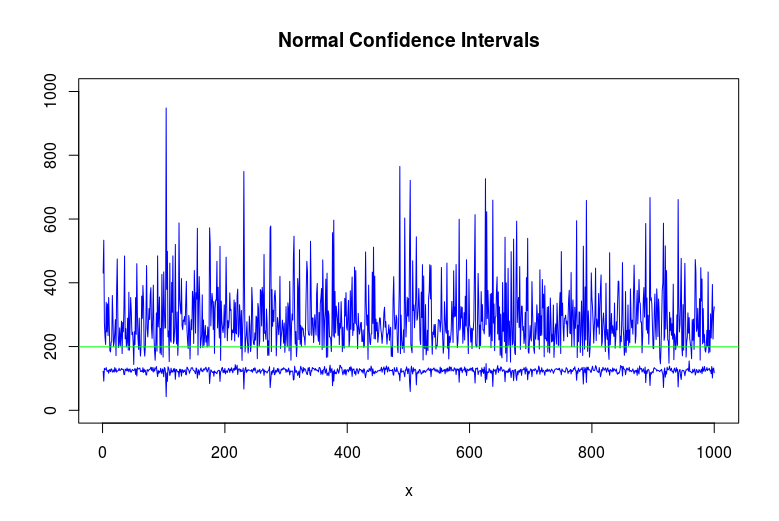
\includegraphics[width=3in]{Assignments/a2/e2-nci.png}}
{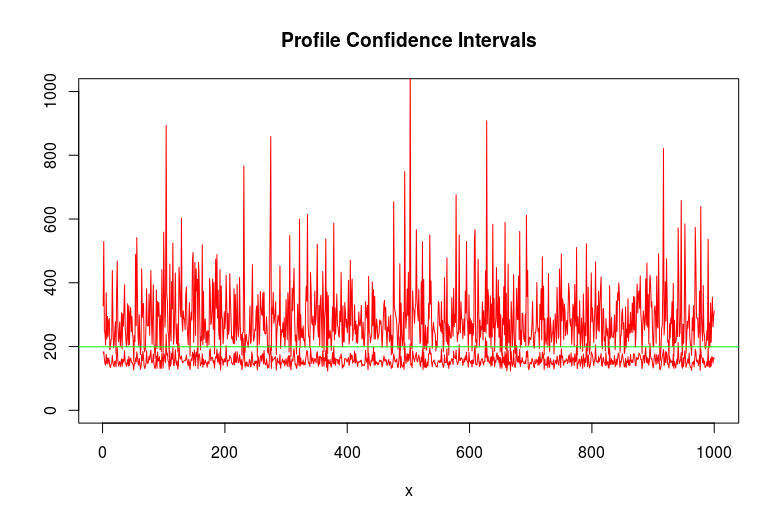
\includegraphics[width=3in]{Assignments/a2/e2-pllci.png}}
\caption{Experiment II confidence intervals for $z_p$(green) given through MLE (blue) and profile likelihood (red) methods. As expected, by choosing to focus on the $0.99^{th}$ quantile rather than the $0.999^{th}$, we see ``calmer" behavior from the upper bound of both these confidence intervals.}

\end{center}
\end{figure}


\section*{Experiment III}
\begin{figure}[H]
\begin{center}
{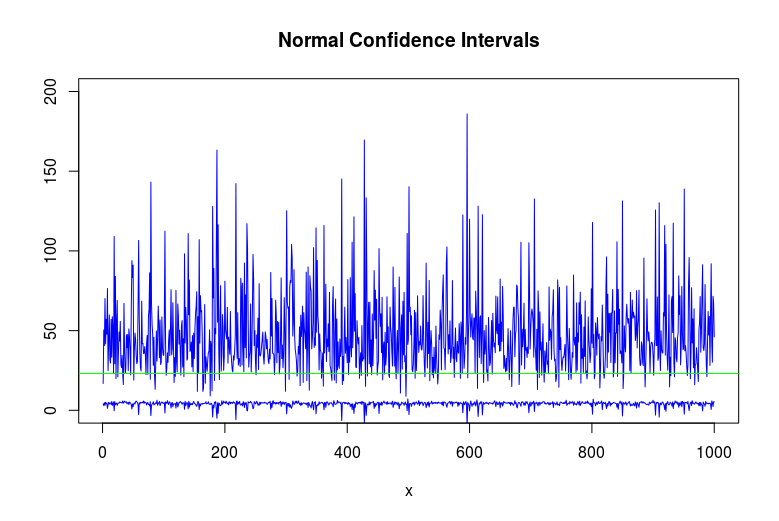
\includegraphics[width=3in]{Assignments/a2/e3-nci.png}}
{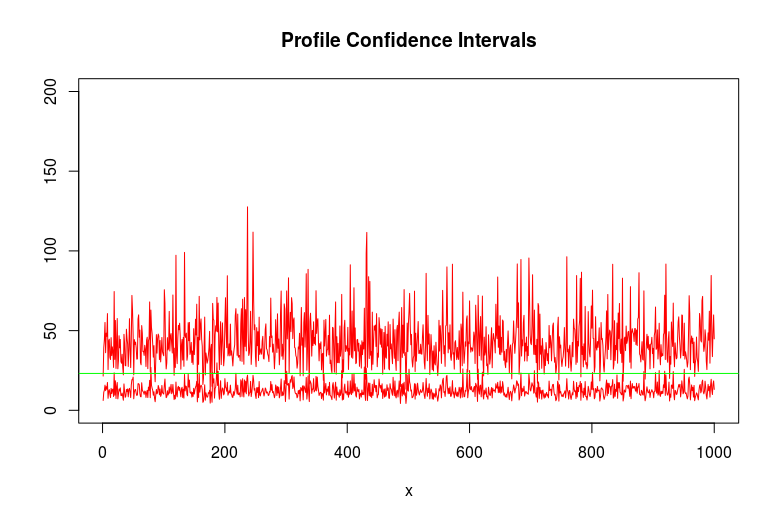
\includegraphics[width=3in]{Assignments/a2/e3-pllci.png}}
\caption{Experiment III confidence intervals for $z_p$(green) given through MLE (blue) and profile likelihood (red) methods. Here we note that the average size of the normal confidence interval seems to be considerably larger than that of the profile confidence interval. We expect both to drop as we move from experiment III to experiment IV and look at a lower quantile.}
\end{center}
\end{figure}

\section*{Experiment IV}
\begin{figure}[H]
\begin{center}
{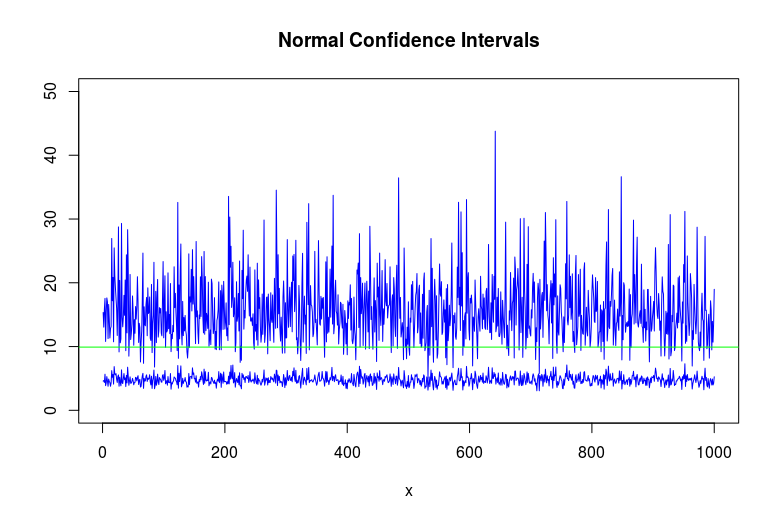
\includegraphics[width=3in]{Assignments/a2/e4-nci.png}}
{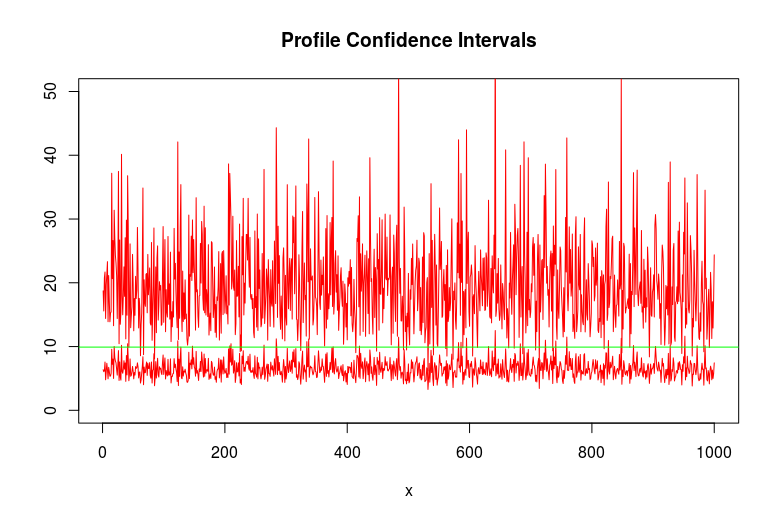
\includegraphics[width=3in]{Assignments/a2/e4-pllci.png}}
\caption{Experiment IV confidence intervals for $z_p$(green) given through MLE (blue) and profile likelihood (red) methods. Surprisingly, in this case, the normal CIs are smaller (on average) than the profile quantiles.}
\end{center}
\end{figure}


\section*{Conclusions}
Below, is a table reporting the hits and misses from each constructed confidence interval. In parenthesis is the method used to derive the confidence interval. L-miss refers to left misses (meaning that our true value $z_p$ is strictly smaller than any point in the interval). R-miss refers to right misses (meaning that our true value $z_p$ is strictly greater than any point in the interval).
\begin{center}
    \begin{tabular}{||c|c|c|c|c|c|c||}\hline
     Exp& Hits (Norm) &Hits (PLL) & L-Miss (Norm) &L-Miss (PLL)& R-Miss (Norm)& R-Miss (PLL)\\\hline
     I& 873 &469 & 0&12 &127 & 519 \\\hline
     II&   865 &864 & 0& 19& 135& 117\\\hline
     III& 891 &933 &0 &27 &109 & 40 \\\hline
     IV&  906  &936 &0 & 31&94 & 33\\\hline
\end{tabular}
\end{center}

We note here that although the two sided confidence interval should miss equally from either side, the normal confidence interval never misses from the left. As $n$ gets larger, we see that the proportion of left misses grows closer to that of right misses. Of course, as we are approximating a $z_p$ with $p\in \{0.99, 0.999\}$, we might expect to see fewer left misses since the approximated value is a high valued quantile (of an extreme distribution). As the normal interval is symmetric around our estimate $\hat{z}_p$ (which we hope is a good one), it follows that low variance estimates will most likely yield confidence intervals that will never miss from the left.  


\begin{center}
    \begin{tabular}{||c|c|c||}\hline
    \multicolumn{3}{||c||}{Mean Confidence Interval Width}\\\hline\hline
     Exp& Mean CI size (Norm) & Mean CI size (PLL) \\\hline
     I&  776.81&163.83   \\\hline
     II&  165.45&134.76  \\\hline
     III&43.53 &30.68 \\\hline
     IV& 10.95& 13.23  \\\hline
\end{tabular}
\end{center}
When we look at the average confidence width, we note that difference in performances between the normal CI and the pll CI in the first experiment can be greatly explained by the width of the average normal confidence interval. The variance retrieved fro $\hat{z}_p$ from the delta method is too large and that show us that the model is not actually certain of the true value $z_p$. So while the confidence intervals derived from this method perform well, they are too large to be regarded as having statistical power.

Finally, we note that, as $n$ grows the coverage of $z_p$ by the profile confidence interval gets closer (and faster) to the expected value of $95\%$ than the coverage given by the normal confidence interval.
\end{solution}



\end{document}

